\documentclass[11pt, a4paper, titlepage]{article}

% packages

\usepackage[utf8]{inputenc}
\usepackage[T1]{fontenc}

\usepackage{amsmath}
\usepackage{amsfonts}
\usepackage{amssymb}
\usepackage{setspace}
\usepackage{wrapfig}
\usepackage{cite}
\usepackage{indentfirst}
\usepackage{subcaption}

%% packages and package-dependent commands

\usepackage{graphicx}
\graphicspath{{./images/}}

\usepackage[thmmarks]{ntheorem}

\theorembodyfont{\normalfont}
\theoremseparator{.}
\theoremindent0.5cm
\theoremnumbering{arabic}
\theoremsymbol{\ensuremath{\ast}}
\newtheorem{definition}{Definition}

\usepackage{xargs}

\usepackage[pdftex, dvipsnames, hyperref]{xcolor}

\definecolor{mnk_blue}{rgb}{.2, .56, 1}
\definecolor{mnk_red}{rgb}{.9, .16, .1}
\definecolor{mnk_orange}{rgb}{.99, .59, .12}
\definecolor{mnk_yellow}{rgb}{.9, .86, .45}

\makeatletter
\usepackage[pdfusetitle]{hyperref}
\hypersetup{colorlinks, urlcolor=mnk_blue, citecolor=black, filecolor=black,
            linkcolor=black, linktoc=page,
            pdfsubject={Algorithms on graphs; Persistent Phylogeny}}
\makeatother

\usepackage[
  colorinlistoftodos,
  prependcaption,
  backgroundcolor=mnk_yellow,
  linecolor=mnk_yellow,
  textsize=tiny
]{todonotes}

\newcommandx{\fix}[2][1=]{%
  \todo[backgroundcolor=mnk_red, linecolor=mnk_red, #1]{#2}
}

\newcommandx{\wip}[2][1=]{%
  \todo[backgroundcolor=mnk_orange, linecolor=mnk_orange, #1]{#2}
}

\usepackage{tikz}

\usepackage{relsize}

\newcommand*{\cc}{%
  C\nolinebreak[4]\hspace{-.05em}%
  \raisebox{.4ex}{\relsize{-3}{\textbf{++}}}%
}

\newcommandx*{\m}[2][1, 2]{\ensuremath{{M_{#1}}_{#2}}}
\newcommand*{\ma}{\ensuremath{(M, A)}}

\newcommand*{\species}[1][]{\ensuremath{s_{#1}}}
\newcommand*{\character}[1][]{\ensuremath{c_{#1}}}

\newcommand*{\g}{\ensuremath{G}}
\newcommand*{\grb}{\ensuremath{G_{RB}}}
\newcommand*{\edge}[2]{\ensuremath{(#1, #2)}}

% information

\author{Davide Casella}
\title{Efficient algorithms to compute a Persistent Phylogeny}

% body

\begin{document}
  \hypersetup{pageanchor=false}

  %!TEX root = ../thesis.tex

\begin{titlepage}

  \begin{spacing}{1.48}
    \begin{wrapfigure}[5]{l}[20mm]{0.2\linewidth}
      \includegraphics[width=\linewidth]{bicocca.png}
    \end{wrapfigure}
    \text{} \\[-0.027\textheight]
    Università degli Studi di Milano Bicocca \\
    \textbf{Scuola di Scienze} \\
    \textbf{Dipartimento di Informatica, Sistemistica e Comunicazione} \\
    \textbf{Corso di laurea in Informatica}
  \end{spacing}

  \vfill

  \begin{spacing}{2}
    \begin{center}
      {\huge \textbf{Efficient approaches to the persistent phylogeny}}
    \end{center}
  \end{spacing}

  \vfill

  \begin{onehalfspace}
    \begin{flushleft}
      {\large
        \textbf{Relatore:} \textit{Prof. Paola Bonizzoni} \\
        \textbf{Co-relatore:} \textit{Prof. Gianluca Della Vedova}
      }
    \end{flushleft}
  \end{onehalfspace}

  \vfill

  \begin{onehalfspace}
    \begin{flushright}
      {\large
        \textbf{Relazione della prova finale di:} \\
        \textit{Davide Casella} \\
        \textit{Matricola 793631}
      }
    \end{flushright}
  \end{onehalfspace}

  \vfill

  \begin{center}
    {\large \textbf{Anno Accademico 2016--2017}}
  \end{center}

\end{titlepage}


  %!TEX root = ../thesis.tex

\begin{abstract}

  Recently it has become increasingly important to study character-based phylogeny models that allow for loss of characters.
  For example, tumor phylogeny often involves the loss of previously acquired mutations following the deletion of entire genomic regions.

  The Persistent Phylogeny model solves this by generalizing the concept of Perfect Phylogeny, allowing for each character to be acquired and lost at most once in the evolutionary history.

  The first polynomial time algorithm for reconstructing a Persistent Phylogeny tree starting from a binary matrix was introduced very recently.
  In this thesis we describe the process behind the implementation of said algorithm, using the \cc{} language and Boost libraries.

\end{abstract}


  \tableofcontents
  \thispagestyle{empty}

  \pagebreak

  \listoftodos          % temporary - delete
  \thispagestyle{empty} % temporary - delete
  \pagebreak            % temporary - delete

  \hypersetup{pageanchor=true}
  \setcounter{page}{1}

  %!TEX root = ../thesis.tex

\section{Introduction}\label{section:introduction}

\todo[inline]{Expand}

Reconstructing character-based phylogenies, which are used to study the evolution of characters shared by a collection of species (taxa or individuals), \todo{Citation needed} is a recurring problem in Bioinformatics, mainly due to the complexity of the task. In fact, \todo{Citation needed} there exist multiple approaches to evolutionary history reconstruction; \todo{Citation needed} most of those approaches try to reduce the problem by limiting the way (or amount of times) characters can change state in the phylogenetic tree \cite{PPptime1994}. \todo{Citation needed} The Persistent Phylogeny model, which we will talk about in the following sections, allows characters to be acquired and lost at most once in the evolutionary history.

\subsection{Character evolution in Bioinformatics}\label{section:character-evolution}

\todo[inline]{Expand}

To study the state changes of characters in an evolutionary tree we can represent species and their characters as rows and columns of a matrix; each element of the matrix marks the specific state of a character for a species.

We will consider the case in which all characters are binary, making them able to assume only one of two states, 0 or 1. For each species, the state of a character represents if the species has or doesn't have a given feature.

\todo{Citation needed} Binary phylogeny models have already been explored and \dots
\wip[inline]{Continue}

\begin{definition}\label{definition:m}
  \m{} is a $n \times m$ binary matrix over a set $m$ of characters and a set $n$ of species.

  \m[i][j] represents the state of a character \character[j] for a species \species[i].
\end{definition}

A matrix \m{} can then be represented as an undirected bipartite graph. The set of vertices of the graph is $V = S \cup C$, where $S$ is the set of species and $C$ the set of characters.

\begin{figure}[h]
  %!TEX root = ../thesis.tex

\begin{subfigure}[b]{0.45\textwidth}
  \centering
    \begin{tabular}{c | c c c c}
      \m{}  & $c_0$ & $c_1$ & $c_2$ & $c_3$ \\ \hline
      $s_0$ & 0     & 1     & 1     & 1     \\
      $s_1$ & 0     & 0     & 0     & 1     \\
      $s_2$ & 1     & 1     & 0     & 0     \\
      $s_3$ & 1     & 0     & 1     & 0
    \end{tabular}

  \caption{Matrix for the instance}\label{figure:1:a}
\end{subfigure}
\hfill
\begin{subfigure}[b]{0.45\textwidth}
  \centering
    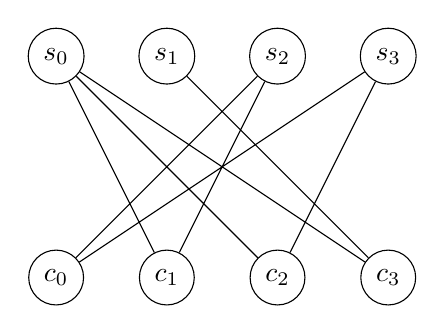
\begin{tikzpicture}
      {\tikzstyle{every node}=[circle, draw]
        \foreach \i in {0, ..., 3}
        {
          \node (s\i) at (\i*40pt, 80pt) {\species[\i]};
        }

        \foreach \j in {0, ..., 3}
        {
          \node (c\j) at (\j*40pt, 0) {\character[\j]};
        }
      }

      \draw
        (c0) -- (s2)
        (c0) -- (s3)
        (c1) -- (s0)
        (c1) -- (s2)
        (c2) -- (s0)
        (c2) -- (s3)
        (c3) -- (s0)
        (c3) -- (s1);
    \end{tikzpicture}

  \caption{Graph for the instance}\label{figure:1:b}
\end{subfigure}


  \caption{An instance of a character-based phylogeny represented as matrix and graph $(\text{4 species} \times \text{4 characters})$}\label{figure:1}
\end{figure}

In the figure above (\ref{figure:1}) we have a set of species $S = \{ \species[0], \species[1], \species[2], \species[3] \}$ and a set of characters $C = \{ \character[0], \character[1], \character[2], \character[3] \}$.
Each element $\m[i][j] = 1$ of the matrix (\ref{figure:1:a}) is shown as the edge \edge{\species[i]}{\character[j]} in the corresponding graph (\ref{figure:1:b}).

\subsubsection{Character states}\label{section:character-states}

\todo[inline]{Expand}

In a phylogenetic tree, characters can be acquired and lost; we will use the notation \character[][+] for acquired characters and \character[][-] for lost characters. Each \character[][+] and \character[][-] represents a \emph{signed} character.

The Persistent Phylogeny model enables characters to be lost at most once in the evolutionary events; we then need a way to keep track of the characters that were previously acquired. This is solved by introducing the concept of \todo{Citation needed?} \emph{active} characters.

Active characters are a subset of the instance's current set of characters $C = \{ \character[0], \dots, \character[m-1] \}$.
A character becomes active whenever it is gained in the tree.

\subsection{Persistent Phylogeny problem}\label{section:ppp}

\wip[inline]{Expand}

A Persistent Phylogeny can also be called Persistent Perfect Phylogeny (P-PP, or simply put, PPP), since its model is directly related to that of the Perfect Phylogeny.

Each instance of a PPP is associated to a pair \ma{} and a rooted tree $T$, where $T$ is a \emph{persistent phylogeny} for the pair \ma{}. \fix{Reword? Too many repetitions} If \ma{} admits a persistent phylogeny we then say that the matrix $M$ is solved by the tree $T$ \cite{PPPptime2016,PPPcgraph2016}.

We now formalize input and output parameters for the Persistent Phylogeny problem \cite{PPPptime2016}.

\begin{definition}[Persistent Phylogeny problem]\label{definition:ppp}
  \text{}

  \textit{Input:} pair \ma{} where \m{} is a $n \times m$ binary matrix over a set of $m$ characters and a set of $n$ species, and A is a subset of its characters.

  \textit{Output:} tree $T$ solving \m{} if it exists.
\end{definition}

\todo[inline]{Add more?}

\subsubsection{Red-black graph representation}\label{section:grb}

A red-black graph for an instance of PPP is an undirected bipartite graph whose edges are colored as either red or black.

\begin{definition}[Red-black graph for PPP]\label{definition:grb}
  Let $S$ be a set of species vertices, $C$ a set of character vertices, $B$ a set of black edges and $R$ a set of red edges.
  Then \grb{} is defined as follows:

  \[ \grb{} = (S \cup C, B \cup R) \]

  The vertex set $V$ of \grb{} is formally represented as two disjoint and independent sets $S$ and $C$.

  The edge set $E$ of \grb{} is formally represented as two disjoint and independent sets $B$ and $R$.
\end{definition}

The set of characters adjacent to a species \species{} is denoted as $C(\species{})$. Conversely, we use $S(\character{})$ to indicate the set of species adjacent to a character \character{}.

A character \character{} is \emph{inactive} in \grb{} if all of its incident edges are black. Conversely, \character{} is \emph{active} in \grb{} if all of its incident edges are red.

A character \character{} is \emph{universal} in \grb{} if it's inactive and its set $S(\character{})$ is made up of all the species in the connected component that contains \character{}. Moreover, \character{} is \emph{free} in \grb{} if it's active and $S(\character{})$ is made up of all the species in the connected component that contains \character{}.

We say that a red-black graph \grb{} is solved by a tree $T$ if $T$ is a persisteny phylogeny for the graph. Moreover, the construction of a tree $T$ can be expressed as a series of graph operations performed on the red-black graph.
This sequence of operations is called \emph{c-reduction}; a c-reduction is then called \emph{successful c-reduction} if, when applied to a red-black graph that admits a persistent phylogeny, results in an empty graph.

Each graph operation in a c-reduction, represented as a signed character, is called a \emph{realization}.

\begin{definition}[Realization]\label{definition:realization}
  Let \grb{} be a red-black graph and \character{} a character of \grb{}.
  Let $Conn(\character{})$ be the set of species of \grb{} in the connected component that contains \character{}.

  The realization of \character[][+] on \grb{}, which is feasible only if \character{} is inactive, involves adding red edges between \character{} and each species in $Conn(\character{}) \setminus S(\character{})$ and deleting all black edges incident on \character{}.

  The realization of \character[][-] on \grb{}, which is feasible only if \character{} is active and there is no species in $Conn(\character{}) \setminus S(\character{})$ (i.e., \character{} is free), involves deleting all (red) edges incident on \character{}.

  After a realization is performed on \grb{}, all isolated vertices of \grb{} may be deleted.
\end{definition}

The realization of a species \species{} is defined as the realization of each character in $C(\species{})$ in any order.

The notion of c-reduction was first introduced in \cite{PPPbin2012} and is defined as a sequence of positive characters \character[][+]. A c-reduction $R$ is \emph{feasible} for \grb{} if the realization of each signed character in $R$ is feasible for the current state \fix{Reword?} \grb{} is in, and every time a character \character[i] becomes free the realization of \character[i][-] is applied \cite{PPPcgraph2016}.

A c-reduction $\langle \character[0][\pm], \dots, \character[k][\pm] \rangle$ (where $0$ and $k$ represent the indexes of the signed characters in the sequence) applied to \grb{} produces a graph \grb[k], which represents the state of \grb{} after the realization of the characters from \character[0][\pm] to \character[k][\pm].
The realization of \character[0][\pm] on \grb{} produces \grb[0], while for indexes $i > 0$ each \grb[i] is generated from the realization of \character[i][\pm] applied on \grb[i-1].

We provide an example for a c-reduction being applied to a red-black graph in \hyperref[figure:3]{Figure 3}.

\paragraph{Red \boldmath{\sg{}}s}

For a c-reduction to be successful, the graphs \grb[i] induced by the realization of each signed character \character[i][\pm] must not contain a red \sg{}.

We provide some graphical examples of red \sg{}s below.

\begin{figure}[h]
  %!TEX root = ../thesis.tex

\centering
  \begin{subfigure}[b]{0.98\textwidth}
    \centering
      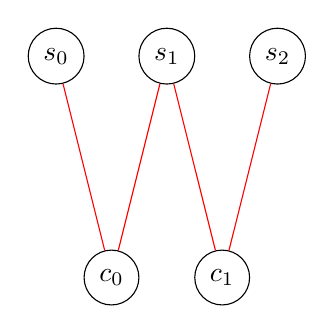
\begin{tikzpicture}
        {\tikzstyle{every node}=[circle, draw]
          \foreach \i in {0, 1, 2}
          {
            \node (s\i) at (\i*40pt, 80pt) {\species[\i]};
          }

          \foreach \j in {0, 1}
          {
            \node (c\j) at (\j*40pt+20pt, 0) {\character[\j]};
          }
        }

        \draw [red]
          (c0) -- (s0)
          (c0) -- (s1)
          (c1) -- (s1)
          (c1) -- (s2);
      \end{tikzpicture}

    \caption{\grb{} being the smallest possible red \sg{}}\label{figure:2:a}
  \end{subfigure}

  \bigskip

  \begin{subfigure}[b]{0.98\textwidth}
    \centering
      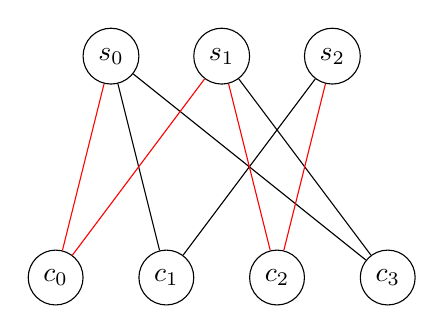
\begin{tikzpicture}
        {\tikzstyle{every node}=[circle, draw]
          \foreach \i in {0, ..., 2}
          {
            \node (s\i) at (\i*40pt, 80pt) {\species[\i]};
          }

          \foreach \j in {0, ..., 3}
          {
            \node (c\j) at (\j*40pt-20pt, 0) {\character[\j]};
          }
        }

        \draw
          (c1) -- (s0)
          (c1) -- (s2)
          (c3) -- (s0)
          (c3) -- (s1);

        \draw [red]
          (c0) -- (s0)
          (c0) -- (s1)
          (c2) -- (s1)
          (c2) -- (s2);
      \end{tikzpicture}

    \caption{\grb[1] containing a red \sg{}}\label{figure:2:b}
  \end{subfigure}

  \bigskip

  \begin{subfigure}[b]{0.98\textwidth}
    \centering
      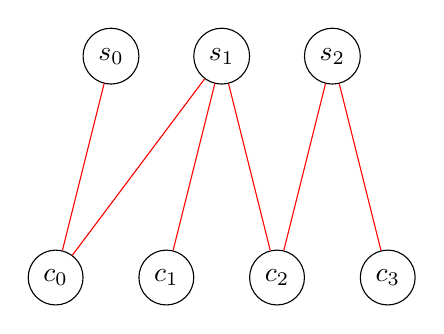
\begin{tikzpicture}
        {\tikzstyle{every node}=[circle, draw]
          \foreach \i in {0, ..., 2}
          {
            \node (s\i) at (\i*40pt, 80pt) {\species[\i]};
          }

          \foreach \j in {0, ..., 3}
          {
            \node (c\j) at (\j*40pt-20pt, 0) {\character[\j]};
          }
        }

        \draw [red]
          (c0) -- (s0)
          (c0) -- (s1)
          (c1) -- (s1)
          (c2) -- (s1)
          (c2) -- (s2)
          (c3) -- (s2);
      \end{tikzpicture}

    \caption{\grb[3] containing a red \sg{} - notice how the graph can't be emptied}\label{figure:2:c}
  \end{subfigure}


  \caption{Examples of red \sg{}s}\label{figure:2}
\end{figure}

We observe in the figure above (\ref{figure:2:a} and \ref{figure:2:c} in particular) that none of the characters are free in \grb{}, making the realization of any \character[i][-] impossible; then, the graph can't be emptied by a c-reduction.

\begin{definition}[Red \sg{}]\label{definition:sigma-graph}
  Let \grb{} be a red-black graph, \character[0] \character[1] two active characters of \grb{} and \species[0] \species[1] \species[2] three species of \grb{}.

  \grb{} contains a red \sg{} if there exists a (red) path $\species[0], \character[0], \species[1], \character[1], \species[2]$ of length 4, and the edges \edge{\character[0]}{\species[2]} and \edge{\character[1]}{\species[0]} do not exist.
\end{definition}

A c-reduction $R$ is successful if, when applied to a red-black graph \grb{}, the graphs \grb[i] induced by the realization of each signed character \character[i][\pm] of $R$ does not contain a red \sg{}.

A red-black graph consisting of \textit{k} connected components has a successful reduction $R$ if and only if each component has a successful reduction $R_{i}$ (with $1 < i < k$). Then $R$ consists of any concatenation of the \textit{k} sequences $R_{i}$ \cite{PPPptime2016}.

\begin{figure}[H]
  %!TEX root = ../thesis.tex

\begin{subfigure}[b]{0.45\textwidth}
  \centering
    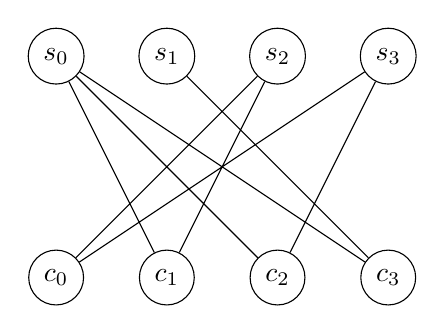
\begin{tikzpicture}
      {\tikzstyle{every node}=[circle, draw]
        \foreach \i in {0, ..., 3}
        {
          \node (s\i) at (\i*40pt, 80pt) {\species[\i]};
        }

        \foreach \j in {0, ..., 3}
        {
          \node (c\j) at (\j*40pt, 0) {\character[\j]};
        }
      }

      \draw
        (c0) -- (s2)
        (c0) -- (s3)
        (c1) -- (s0)
        (c1) -- (s2)
        (c2) -- (s0)
        (c2) -- (s3)
        (c3) -- (s0)
        (c3) -- (s1);
    \end{tikzpicture}

  \caption{\grb{}}
  \label{figure:3:a}
\end{subfigure}
\hfill
\begin{subfigure}[b]{0.45\textwidth}
  \centering
    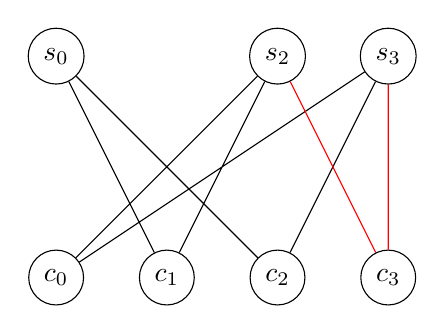
\begin{tikzpicture}
      {\tikzstyle{every node}=[circle, draw]
        \foreach \i in {0, 2, 3}
        {
          \node (s\i) at (\i*40pt, 80pt) {\species[\i]};
        }

        \foreach \j in {0, ..., 3}
        {
          \node (c\j) at (\j*40pt, 0) {\character[\j]};
        }
      }

      \draw
        (c0) -- (s2)
        (c0) -- (s3)
        (c1) -- (s0)
        (c1) -- (s2)
        (c2) -- (s0)
        (c2) -- (s3);

      \draw [red]
        (c3) -- (s2)
        (c3) -- (s3);
    \end{tikzpicture}

  \caption{\grb[0], after realizing \character[3][+]}
  \label{figure:3:b}
\end{subfigure}

\bigskip

\begin{subfigure}[b]{0.45\textwidth}
  \centering
    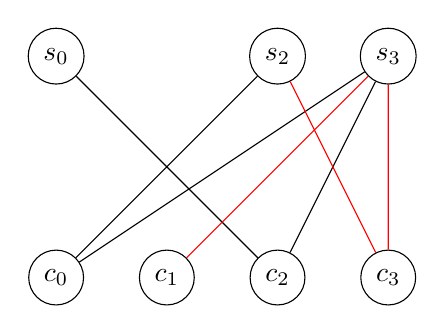
\begin{tikzpicture}
      {\tikzstyle{every node}=[circle, draw]
        \foreach \i in {0, 2, 3}
        {
          \node (s\i) at (\i*40pt, 80pt) {\species[\i]};
        }

        \foreach \j in {0, ..., 3}
        {
          \node (c\j) at (\j*40pt, 0) {\character[\j]};
        }
      }

      \draw
        (c0) -- (s2)
        (c0) -- (s3)
        (c2) -- (s0)
        (c2) -- (s3);

      \draw [red]
        (c1) -- (s3)
        (c3) -- (s2)
        (c3) -- (s3);
    \end{tikzpicture}

  \caption{\grb[1], after realizing \character[1][+]}
  \label{figure:3:c}
\end{subfigure}
\hfill
\begin{subfigure}[b]{0.45\textwidth}
  \centering
    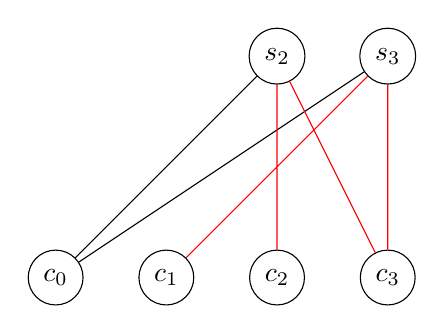
\begin{tikzpicture}
      {\tikzstyle{every node}=[circle, draw]
        \foreach \i in {2, 3}
        {
          \node (s\i) at (\i*40pt, 80pt) {\species[\i]};
        }

        \foreach \j in {0, ..., 3}
        {
          \node (c\j) at (\j*40pt, 0) {\character[\j]};
        }
      }

      \draw
        (c0) -- (s2)
        (c0) -- (s3);

      \draw [red]
        (c1) -- (s3)
        (c2) -- (s2)
        (c3) -- (s2)
        (c3) -- (s3);
    \end{tikzpicture}

  \caption{\grb[2], after realizing \character[2][+]}
  \label{figure:3:d}
\end{subfigure}

\bigskip

\begin{subfigure}[b]{0.45\textwidth}
  \centering
    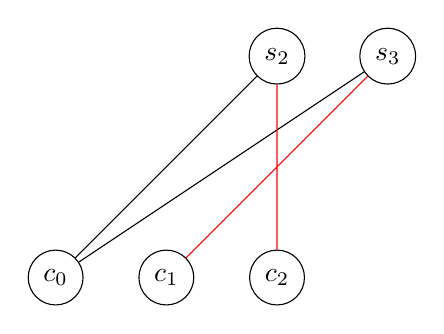
\begin{tikzpicture}
      {\tikzstyle{every node}=[circle, draw]
        \foreach \i in {2, 3}
        {
          \node (s\i) at (\i*40pt, 80pt) {\species[\i]};
        }

        \foreach \j in {0, ..., 2}
        {
          \node (c\j) at (\j*40pt, 0) {\character[\j]};
        }
      }

      \draw
        (c0) -- (s2)
        (c0) -- (s3);

      \draw [red]
        (c1) -- (s3)
        (c2) -- (s2);
    \end{tikzpicture}

  \caption{\grb[3], after realizing \character[3][-]}
  \label{figure:3:e}
\end{subfigure}
\hfill
\begin{subfigure}[b]{0.45\textwidth}
  \centering
    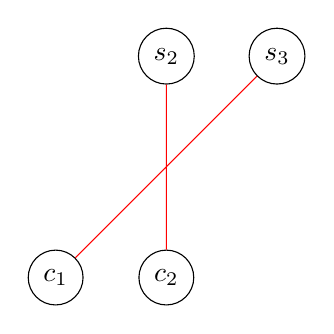
\begin{tikzpicture}
      {\tikzstyle{every node}=[circle, draw]
        \foreach \i in {2, 3}
        {
          \node (s\i) at (\i*40pt, 80pt) {\species[\i]};
        }

        \foreach \j in {1, 2}
        {
          \node (c\j) at (\j*40pt, 0) {\character[\j]};
        }
      }

      \draw [red]
        (c1) -- (s3)
        (c2) -- (s2);
    \end{tikzpicture}

  \caption{\grb[4], after realizing \character[0][+]}
  \label{figure:3:f}
\end{subfigure}

\bigskip

\begin{subfigure}[b]{0.45\textwidth}
  \centering
    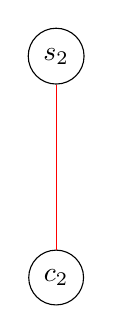
\begin{tikzpicture}
      {\tikzstyle{every node}=[circle, draw]
        \foreach \i in {2}
        {
          \node (s\i) at (\i*40pt, 80pt) {\species[\i]};
        }

        \foreach \j in {2}
        {
          \node (c\j) at (\j*40pt, 0) {\character[\j]};
        }
      }

      \draw [red]
        (c2) -- (s2);
    \end{tikzpicture}

  \caption{\grb[5], after realizing \character[1][-]}
  \label{figure:3:g}
\end{subfigure}
\hfill
\begin{subfigure}[b]{0.45\textwidth}
  \centering
    \begin{tikzpicture}
      {\tikzstyle{every node}=[circle, draw]
        \foreach \i in {}
        {
          \node (s\i) at (\i*40pt, 80pt) {\species[\i]};
        }

        \foreach \j in {}
        {
          \node (c\j) at (\j*40pt, 0) {\character[\j]};
        }
      }
    \end{tikzpicture}

  \caption{\grb[6], after realizing \character[2][-]}
  \label{figure:3:h}
\end{subfigure}


  \caption{Application of a c-reduction $R = \langle \character[3][+], \character[1][+], \character[2][+], \character[3][-], \character[0][+], \character[1][-], \character[2][-] \rangle$ to a red-black graph \grb{}}\label{figure:3}
\end{figure}


  \pagebreak % temporary - delete

  %!TEX root = ../thesis.tex

\section{Algorithm explaination}\label{section:algorithm}

The polynomial-time algorithm introduced in \cite{PPPptime2016} describes a recursive procedure for reducing a red-black graph to an empty graph, if it admits a persistent phylogeny.
The recursion stops either when the base case is reached - empty graph (line \ref{algorithm:reduce:ifempty}) - or when the algorithm can't compute a successful c-reduction for \grb{} - the graph reaches a state of irreducibility (line \ref{algorithm:reduce:ifnosource}).

The procedure for a Reduce function is given below.

\begin{algorithm}[h]\label{algorithm:reduce}
  \caption{Reduce. Recursive reduction of a red-black graph.}

  \SetKwData{Source}{\ensuremath{s}}
  \SetKwData{Sc}{\ensuremath{S_{c}}}
  \SetKwInOut{Input}{Input}
  \SetKwInOut{Output}{Output}

  \Input{Red-black graph \grb{}}
  \Output{c-reduction of the graph \grb{}, if it exists}

  \BlankLine

  Remove singletons from \grb{}\;

  \If{\grb{} is empty}{\label{algorithm:reduce:ifempty}
    \Return $\langle$ $\rangle$\;
  }

  \BlankLine

  \If{\grb{} has a free character \character{}}{
    \grb{} $\gets$ Realize(\character[][-], \grb{})\;

    \Return $\langle$ \character[][-], Reduce(\grb{}) $\rangle$\;
  }

  \BlankLine

  \If{\grb{} has a universal character \character{}}{
    \grb{} $\gets$ Realize(\character[][+], \grb{})\;

    \Return $\langle$ \character[][+], Reduce(\grb{}) $\rangle$\;
  }

  \BlankLine

  \If{\grb{} has k > 1 connected components}{
    \Return $\langle$ Reduce($\grb{}_{0}$), \dots, Reduce($\grb{}_{k-1}$) $\rangle$\;
  }

  \BlankLine

  \gm{} $\gets$ maximal reducible graph of \grb{}\;

  \hasse{} $\gets$ Hasse diagram for \gm{}\;

  \BlankLine

  \If{\hasse{} has no safe source}{\label{algorithm:reduce:ifnosource}
    Abort\;
  }

  \BlankLine

  \Source $\gets$ Find-initial-state(\hasse{})\;

  \Sc $\gets$ sequence of positive characters of \Source that are inactive in \grb{}\;

  \grb{} $\gets$ Realize(\Sc, \grb{})\;

  \BlankLine

  \Return $\langle$ \Sc, Reduce(\grb{}) $\rangle$\;
\end{algorithm}

The Reduce procedure computes signed character realizations with the support of a Realize function, which follows the definition of Realization (\ref{definition:realization}) quite literally. \fix{Reword} We still describe the procedure for the Realize function.

\pagebreak % temporary - delete

\begin{algorithm}[h]\label{algorithm:realize}
  \caption{Realize. Realization of a list of signed characters in a red-black graph.}

  \SetKwData{Lc}{\ensuremath{L_{c}}}
  \SetKwData{Con}{\ensuremath{Conn(\character{})}}
  \SetKwData{Adj}{\ensuremath{S(\character{})}}
  \SetKwInOut{Input}{Input}
  \SetKwInOut{Output}{Output}

  \Input{List of signed characters \Lc of \grb{}}
  \Input{Red-black graph \grb{}}
  \Output{Red-black graph \grb{} after the realization of \Lc, if feasible}

  \BlankLine

  \ForEach{\character[][\pm] $\in$ \Lc}{
    \Con $\gets$ species in the connected component that contains \character{}\;
    \Adj $\gets$ species adjacent to \character{}\;

    \BlankLine

    \If{\character[][+] is inactive}{
      Add red edges between \character{} and each species in $\Con \setminus \Adj$\;

      Delete black edges incident on \character{}\;
    }
    \ElseIf{\character[][-] is active}{
      Delete edges incident on \character{}\;
    }
    \Else{
      Abort\;
    }
  }

  \BlankLine

  \Return \grb{}\;
\end{algorithm}

Notice that a realization may alter the connected components of the red-black graph; we then need to recompute (or update) the connected component of a character \character[][\pm] before its realization.

We will address the Find-initial-state procedure in detail in section \ref{section:safe-chains-sources}.

\subsection{Preparing the graph}\label{section:preparing-the-graph}

\subsection{Maximal reducible graph and Hasse diagram}\label{section:gm-hassediagram}

\subsection{Safe chains and sources}\label{section:safe-chains-sources}


  \pagebreak % temporary - delete

  %!TEX root = ../thesis.tex

\section{Algorithm implementation}\label{section:implementation}

\subsection{Language choices}\label{section:language-choices}

\subsubsection{Boost libraries}\label{section:boost-libs}

\paragraph{Boost Graph}

\paragraph{Boost Bimap}

\paragraph{Boost Program Options}

\paragraph{Boost Python}

\subsection{Program options}\label{section:program-options}

\subsection{Boost Graph classes}\label{section:graph-classes}

\subsubsection{RBGraph class}\label{section:rbgraph-class}

\paragraph{Traits and properties}

\paragraph{General purpose functions}

\paragraph{Algorithm functions}

\subsubsection{HDGraph class}\label{section:hdgraph-class}

\paragraph{Traits and properties}

\paragraph{General purpose functions}

\subsection{Algorithm functions}\label{section:algorithm-functions}

\subsubsection{Realize characters and species}\label{section:realize}

\subsubsection{Find initial state(s)}\label{section:initial-state}

\subsubsection{Reduce}\label{section:reduce}


  \todo[inline]{Add section to talk about the performed tests}

  \pagebreak % temporary - delete

  %!TEX root = ../thesis.tex

\section{Conclusions}\label{section:conclusions}

\subsection{Implementation improvements}\label{section:impl-improvements}

\todo[inline]{Find a better way to X}

\subsubsection{Bottlenecks}\label{section:bottlenecks}

\todo[inline]{Repeated connected components}

\subsection{Further development}\label{section:further-dev}

\todo[inline]{Expand to minimal characters}


  \pagebreak

  \bibliographystyle{abbrv}
  \bibliography{bibliography}
\end{document}
